\chapter{Background and Related Work}

%%%%%%%%%%%%%%%%%%%%%%%%%%%%%%%%%%%%%%%%%%%%%%%%%%%%%%%%%%%%%%%%%%%%%%%%%%

\section{Radiometry Introduction}
Radiometry is the basic terminology to describe light which is crucial to its simulation. First of all, some basic quantities have to be introduced, the related symbols are going to be defined here as well for further use.

\subsection{Important Quantities}

\begin{table}[ht]
\begin{center}
	
	\renewcommand{\arraystretch}{1.2}
	\begin{tabular}{ | l | l | l |}     	
	\hline

	Symbol & Quantity & Unit \\
	\cline{1-3}

	% \(Q_{\lambda}\) 	& 		Spectral radiant energy 		& 		\(J nm^{-1} \) \\
	\(Q\) 			& 		Radiant Energy 				& 		\(j\) \\
	\(\Phi\) 			& 		Radiant flux 					& 		\(W\) \\
	\(I\) 			& 		Radiant intensity 				& 		\(W sr^{-1}\) \\
	\(E\)			&		Irradiance (incident) 			&		\(W m^{-2}\) \\
	\(L\)			&		Radiance						&		\(W m^{-2} sr^{-1}\) \\
	
	\hline

	\end{tabular}
\end{center}
\caption{Important Radiometry Quantities}
\label{tab:radiometry_quantities}
\end{table}

\emph{Radiant energy}, \(Q\), is the energy of a collection of photons which is the basic quantity in lighting.

\emph{Radiant flux} , \(\Phi\), is the time rate of the flow of radiant energy passing through a surface or region of space. Total emission from a light source is generally described in terms of flux. Figure \ref{fig:flux_point_light} shows the flux emitted from a point light source measured by the total amount of energy passing through an virtual sphere around the light.

\begin{figure}[htp]
    \centering
    \fbox{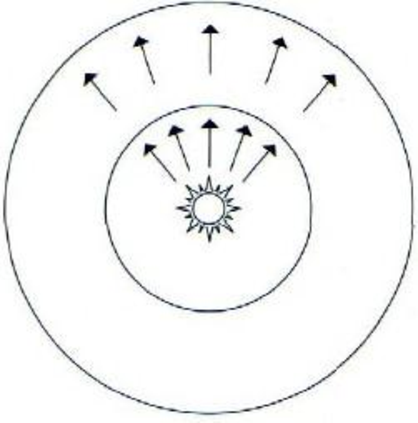
\includegraphics{imgs/flux.pdf}}
    \renewcommand{\thefigure}{\thechapter.\arabic{figure}}
    \caption[Radiant flux of point light source]{Radiant flux from a point light source is passing through the spheres around the light.}
    \label{fig:flux_point_light}
\end{figure}

\emph{Irradiance}, \(E\), is the incident (arriving at a surface location) \emph{radiant flux area density}, which is defined as the differential flux per differential area. While \emph{Radiant exitance} denoted by \(M\) is area density of flux leaving a surface.

\begin{equation}
E(x) = \frac{d\Phi}{dA}
\end{equation}

\emph{Radiance}, \(L\), is the radiant flux per unit solid angle per unit projected area:
\begin{equation}
L(x, \overrightarrow{\omega}) = \frac{d^{2}\Phi}{\cos{\theta} \cdot dA \cdot d\overrightarrow{\omega}}
\end{equation}
where \(x\) is the position and \(\overrightarrow{\omega}\) is the direction.

Radiance is the most important quantity in rendering simulation since it closely represents the color. Also radiance can be considered as the number of photons arriving per time at a small area from a given direction. Radiant energy can be computed by integrating the radiance field over all directions \(\Omega\) and area \(A\).

\begin{equation}
\Phi = \int_{A}\int_{\Omega}L(x, \overrightarrow{\omega})(\overrightarrow{\omega} \cdot \overrightarrow{n})d\overrightarrow{\omega}dx
\label{eq:flux_from_radiance}
\end{equation}

% TF: The following figure should be referenced in the text somewhere.

\begin{figure}[htp]
    \centering
    \fbox{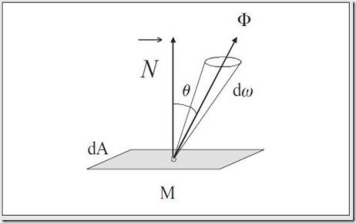
\includegraphics{imgs/radiance_solid_angle.pdf}}
    \renewcommand{\thefigure}{\thechapter.\arabic{figure}}
    \caption[Geometric setup of radiance and solid angle]{Radiance, L, is defined as the radiant flux per unit solid angle, \(\overrightarrow{\omega}\), per unit projected area, \(dA\)}
    \label{fig:radiance_solid_angle}
\end{figure}

%%%%%%%%%%%%%%%%%%%%%%%%%%%%%%%%%%%%%%%%%%%%%%%%%%%%%%%%%%%%%%%%%%%%%%%%%%

\section{Fundamentals of Global Illumination}
With the basic knowledge of radiometry, we will introduced a theoretical framework as the basis of global illumination. There are several components are included in this framework, light source, reflectance and visibility. We will look at these components firstly and then move on to the rendering equation describing the interaction between light and an surface with no participating media.

\subsection{Light Source}
As the light in the form of photons is emitted from light sources initially, the lighting becomes an essential input of the model. There are several types of light sources widely used in Computer Graphics such as point, directional and area lights. The radiance of lighting emitted from light sources is denoted as \( L_{e} \).

We can measure the intensity of light source in \emph{wattage}. Take a point light source for example, the power this light can emit is denoted by \(\Phi\), the emitted light distributes uniformly in all directions, and the irradiance, \(E\), can be computed at a surface as:
\begin{equation}
E(x) = \frac{\Phi \cos{\theta}}{4\pi r^{2}}
\end{equation}
where \(r\) is the distance from \(x\) to the light source and \(\theta\) is the angle between the surface normal and the direction to the light source. From the equation we can intuitively tell a surface facing the source will receive more photons per area than a surface that is oriented differently.

\subsection{Reflectance}
\begin{figure}[htp]
    \centering
    \fbox{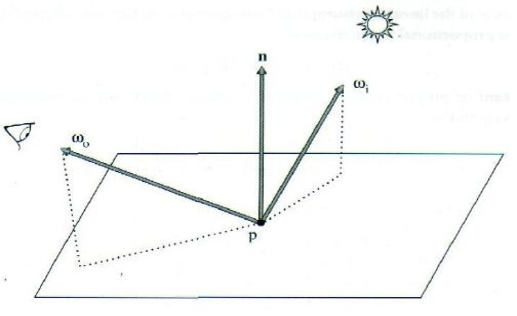
\includegraphics{imgs/brdf.pdf}}
    \renewcommand{\thefigure}{\thechapter.\arabic{figure}}
    \caption[Geometric setup of BRDF]{The geometric setup of BRDF. }
    \label{fig:brdf}
\end{figure}

The \emph{Bidirectional Reflectance Distribution Function}, BRDF, is the mathematic tool describing the reflection of light encounters an surface. To define the BRDF, the geometric configuration is shown in figure \ref{fig:brdf}. \(\omega_{i}\) is the incident lighting direction, \(\omega_{o}\) is the direction in which the reflected light leaving from the surface, and \(n\) is the normal vector at the location \(p\) on the surface. Given the incident radiance \(L_{i}(p, \omega_{i})\), we can find the outgoing radiance to the viewer, \(L_{o}(p, \omega_{o})\).

The BRDF, \(f_{r}\), defines the relationship between differential reflected radiance and differential irradiance:
\begin{equation}
f_{r} = \frac{dL_{o}(p, \omega_{o})}{dE(p, \omega_{i})} = \frac{dL_{o}(p, \omega_{o})}{L_{i}(p, \omega_{i})(\omega_{i} \cdot n)d\omega{i}}
\label{eq:brdf}
\end{equation}

There are two important properties of BRDF used in rendering. The first one is the Helmholtz's law of reciprocity, that is given any pair of directions \( (\omega_{i}, \omega_{o} ) \), we have:
\begin{equation}
f_{r}(p, \omega_{i}, \omega_{o}) = f_r(p, \omega_{o}, \omega_{i})
\end{equation}

Another important physical property of BRDF is energy conservation, stating that the total reflected energy is less than or equal to the incident energy. For all direction \( \omega_{o} \),
\begin{equation}
 \int_{\Omega}f_{r}(p, \omega_{i}, \omega_{o})L_{i}(p, \omega_{i})(\omega_{i} \cdot n)d\omega_{i} \leq 1 , \forall \omega_{i}
\end{equation}

Note that there are special cases exists in the BRDF model, one is the \emph{Lambertian} BRDF in which the outgoing direction is independent from the incident direction. Another extreme case is the perfect mirror reflection BRDF which is a Dirac delta function making the incident direction \(\omega_{i}\) mirrored at the surface normal at the \(p\) on the surface. BRDF including these two special cases is often broadly classified as directional diffuse, and glossy and specular.

Given the definition of BRDF, we can introduce the basic rendering equation, also known as \emph{local illumination model} by integrating the equation \ref{eq:brdf} over the sphere of incident directions around location \(p\), the left side of the equation will be the outgoing radiance in direction \(\omega_{o}\).
\begin{equation}
L_{o}(p, \omega_{o}) = \int_{\Omega}f_{r}(p, \omega_{i}, \omega_{o})L_{i}(p, \omega_{i})(\omega_{i} \cdot n)d\omega_{i}
\label{eq:local_render_equation}
\end{equation}
where \(\Omega\) is the hemisphere of incoming directions at \(p\).

\subsection{Visibility}
Another important component is the visibility computation.
% TF: Add a bit of discussion regarding visibility. I.e., what is it in general terms and why important for lighting.
It is often modeled as a binary function denoted by \(V(x, x')\).
We have following equation:

  \begin{equation}
    V(x, x')=\left\{
    \begin{array}{ll}
      1  & \text{x and x' are mutually visible} \\
      0  & \text{otherwise}
    \end{array}
    \right.
  \end{equation}

Ray casting is the most widely used operator to determine the closest surface in a direction by shooting a ray into the scene trying to find the closest intersection point with the surface. We will discuss ray casting and ray tracing technique further in section \ref{sec:mc_rt}.

Another more complicated model of visibility is the non-binary function occurs between a surface point and an area light source, this model is used to simulate the soft shadows.  \cite{Hasenfratz2003} is a full survey of existing shadow methods dedicated to real-time rendering of soft shadows.

\subsection{Light Transport Equation}

The local rendering equation used to describe the direct lighting effect is too simple for simulating real-world lighting effect, so indirect lighting has to be introduced to this model as well. We introduce the Light Transport Equation (LTE) in this section to form the mathematical basis for all global illumination algorithms. The LTE is also known as the Rendering Equation (RE) which is introduced in the first time in \cite{Kajiya:1986:RE:15922.15902}. We use the LTE term here to be distinguished from the local rendering equation, also it is more suitable with context of global illumination. The LTE states that the outgoing radiance \(L_{o}\) at location \(p\) on the surface in the direction \(\omega_{o}\) is the sum of emitted radiance \(L_{e}\) and reflected radiance \(L_{r}\). The reflected radiance can be computed using the local rendering equation \ref{eq:local_render_equation} so we have final LTE as shown in equation \ref{eq:lte}.

\begin{equation}
L_{o}(p, \omega_{o}) = L_{e}(p, \omega_{o}) + \int_{\Omega}f_{r}(p, \omega_{i}, \omega_{o})L_{i}(p, \omega_{i})(\omega_{i} \cdot n)d\omega_{i}
\label{eq:lte}
\end{equation}

%%%%%%%%%%%%%%%%%%%%%%%%%%%%%%%%%%%%%%%%%%%%%%%%%%%%%%%%%%%%%%%%%%%%%%%%%%

\section{Global Illumination Techniques}
In this section, we will review the several the most popular approaches to compute the global illuminations including radiosity, Monte Carlo ray tracing and photon mapping, and the previous work related to these approaches.

\subsection{Radiosity}

Radiosity, also known as finite element approach, is a classic solution to solving the LTE. It was introduced by  \citeauthor{Goral:1984:MIL:964965.808601} in \citep{Goral:1984:MIL:964965.808601} and has became an active field that was drawn quite a bit of research interest. The underlying idea is to tessellate the surfaces into finite small sub-surfaces called patches as geometric primitives and solve the LTE with them. Solving the LTE using radiosity requires several input. First of all the radiosity value for diffuse surfaces or the BRDF for the non-diffuse surfaces need to be stored for all the patches in the scene. Then it requires a known linear system of equations called form factors which denote the amount of light transport between two patches.

% TF: A picture would help.

Computing the form factors is the most time consuming part because of the initial time complexity of \(O(n^{2})\) of linking \(n\) patches, however when this pre-computation is done the entire scene can be rendered very efficiently. Therefore a lot researchers have focused on minimizing this performance hit. \citeauthor{Hanrahan:1991:RHR:127719.122740} \cite{Hanrahan:1991:RHR:127719.122740} introduced a technique that constructs a hierarchical representation of the form factor matrix to reduce the computation. \citeauthor{Holzschuch94anefficient} \cite{Holzschuch94anefficient} followed a hierarchical structure and introduced a progressive refinement strategy resulting the form factor only being computed when needed to evaluate the energy transfers from a given surface.


\subsection{Ray Tracing}
\label{sec:mc_rt}

\begin{figure}[ht]
    \centering
    \fbox{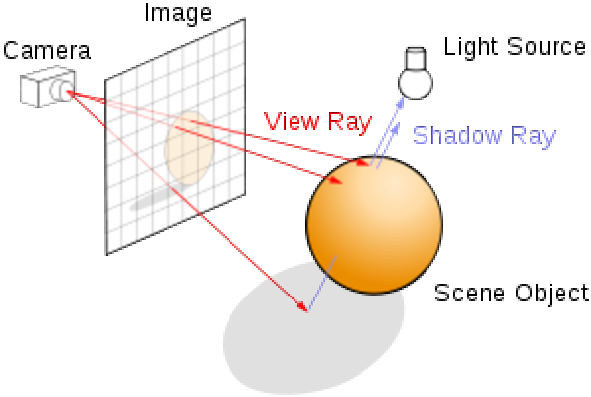
\includegraphics{imgs/ray_tracing.pdf}}
    \renewcommand{\thefigure}{\thechapter.\arabic{figure}}
    \caption[Ray Tracing System Configuration]{A basic configuration of ray tracing rendering system.}
    \label{fig:ray_tracing}
\end{figure}

The classic ray tracing technique became popular in Computer Graphics since 1980 with an introduction of the recursive ray-tracing algorithm by Whitted \cite{Whitted1980}. It is an elegant and simple algorithm for easily rendering shadows and specular surfaces.

The ray tracing algorithm can be broke down into two stages: intersection query and shading. In the first stage, as shown in figure \ref{fig:ray_tracing}, for each pixel on our viewing plane, one or more rays (if the multi-sampling is enabled, this allows for better image quality) are shot into the scene. Those rays directly from the observer are \emph{primary rays}. Then we try to find intersection point along each of the rays with the closest object to the observer. In the shading stage, at each intersection point the direct illumination is computed based on the BRDF determined by the surface material. The computed radiance is converted to the color of the corresponding pixel. The visibility of the light sources can be evaluated with shadow rays.
% TF: Explain how shadow rays work.
If the surface material is specular then a specular ray is traced in the reflected or transmitted direction. The indirect illumination can be computed by spawning and tracing reflected or refracted rays (called \emph{secondary rays}) from the intersection points and repeating the ray tracing recursively.

Ray tracing is not a full global illumination algorithm since it cannot handle the computation of the indirect illumination on diffuse surfaces; it can only compute the illumination for perfect specular material by tracing a ray in the refracted or mirror direction. To simulate the phenomena such as soft shadows, it is necessary to employ Monte Carlo sampling techniques\cite{Kajiya:1986:RE:15922.15902}.

\begin{figure}[htp]
\begin{center}
    \fbox{\subfigure[]{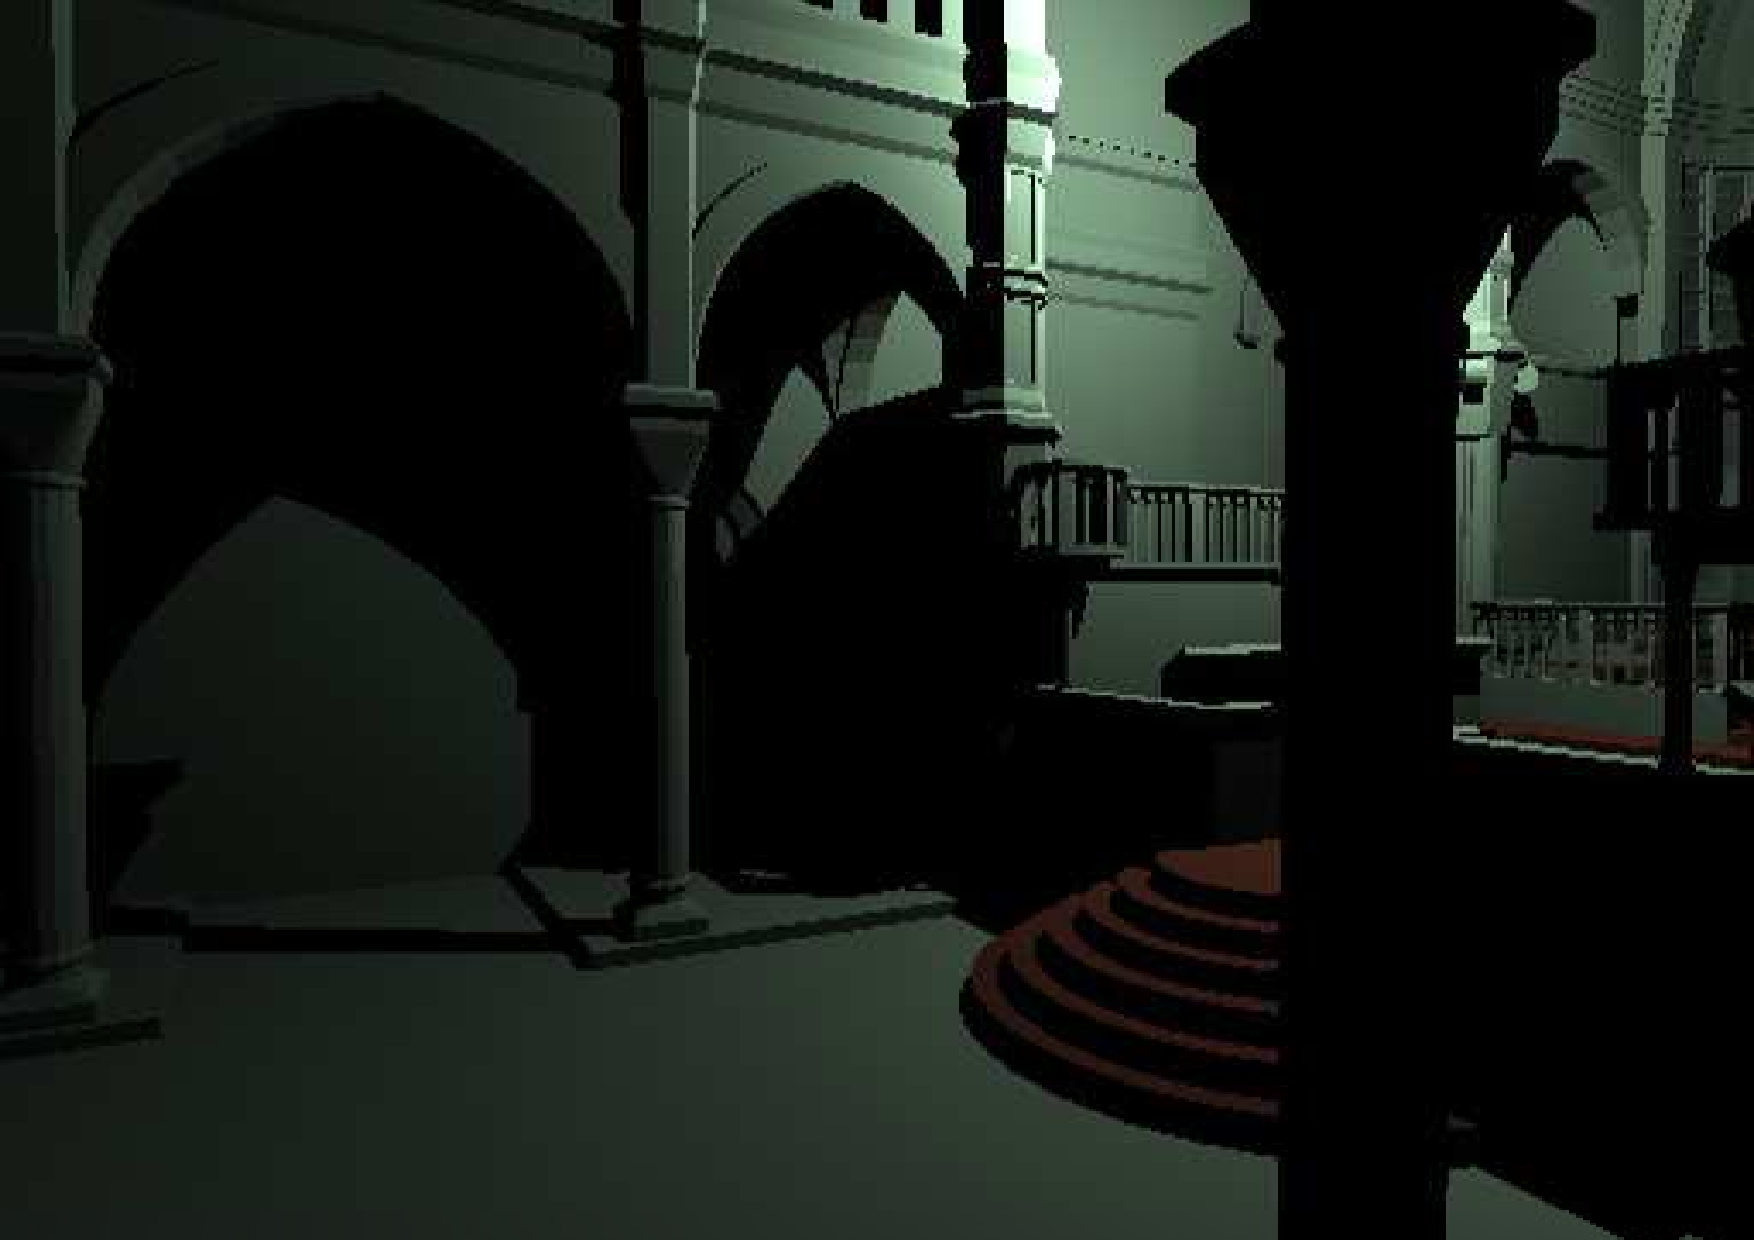
\includegraphics[scale=0.25]{imgs/rt_01.pdf} \subfigure[]{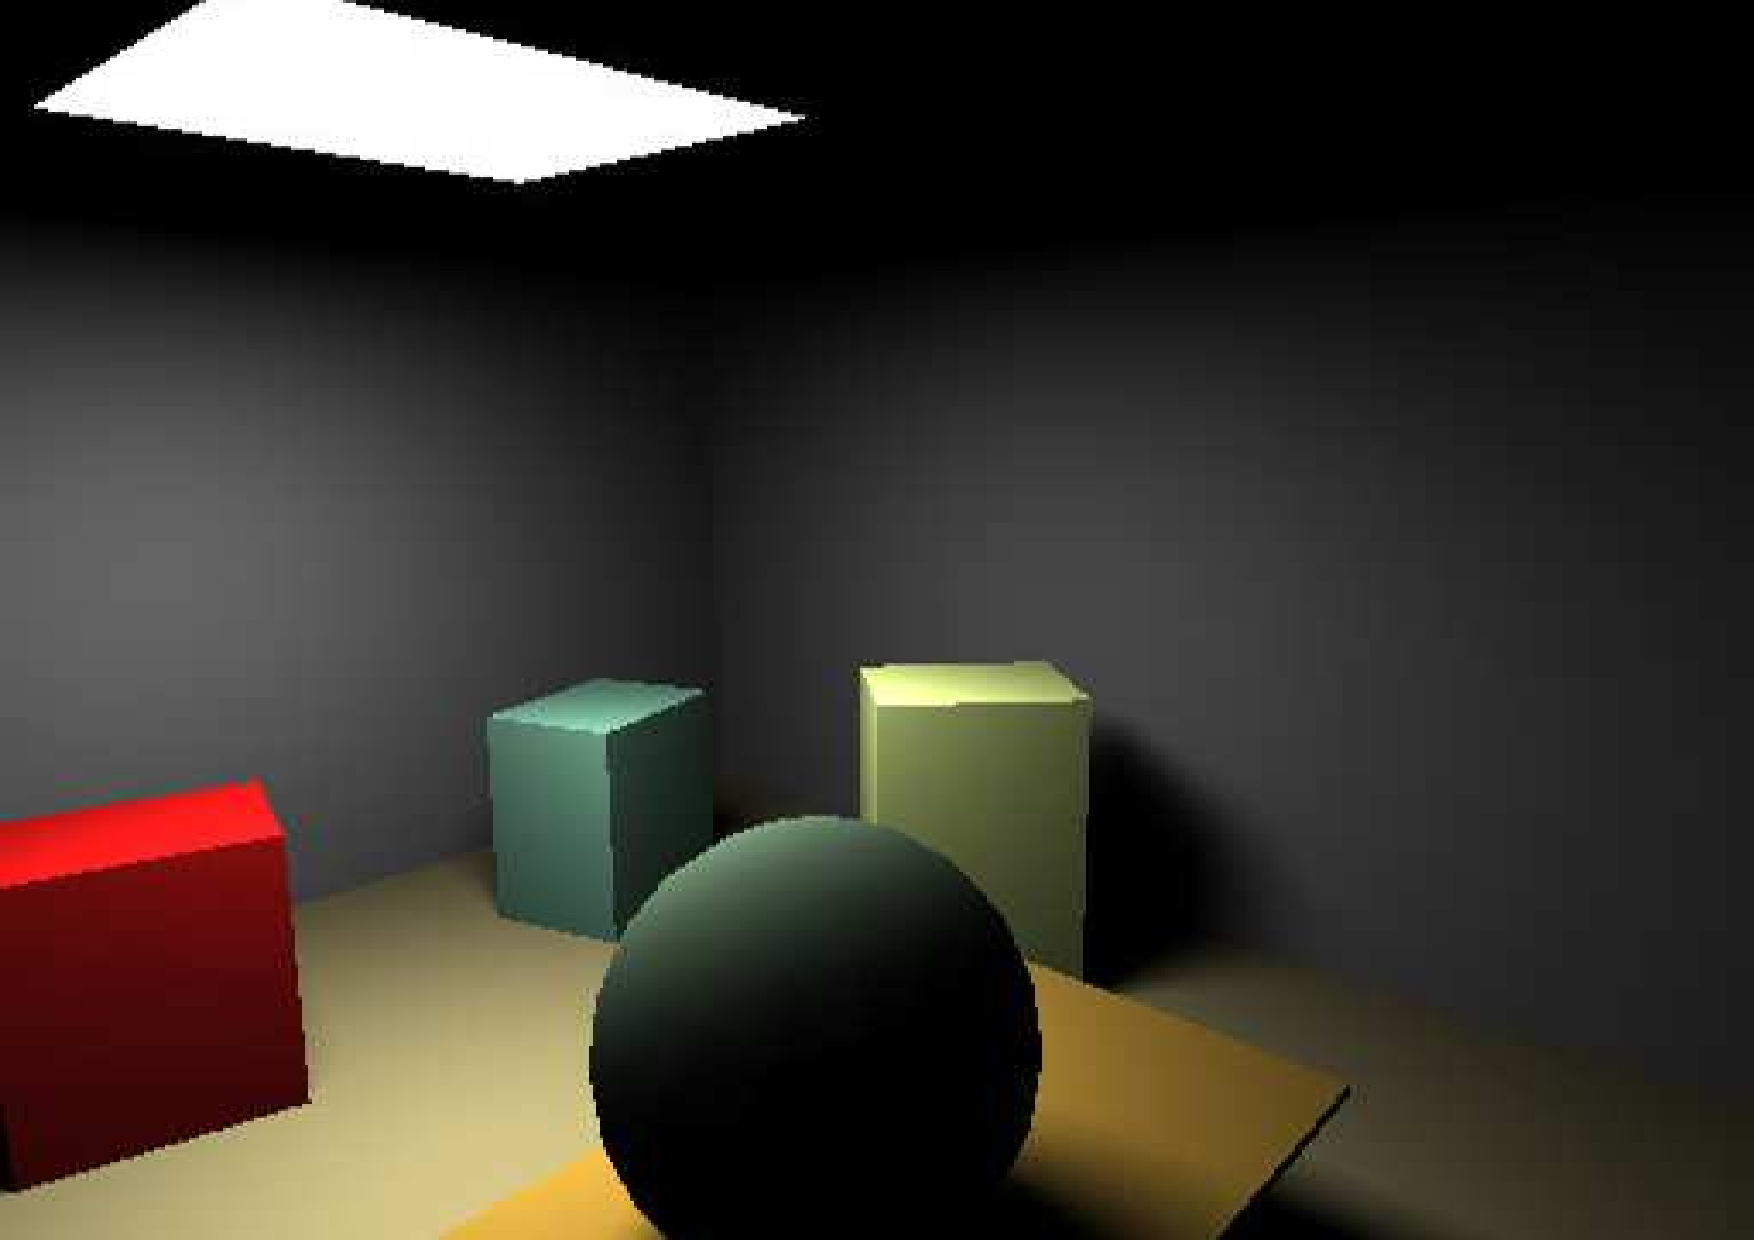
\includegraphics[scale=0.25]{imgs/rt_02.pdf}}}}
    \renewcommand{\thefigure}{\thechapter.\arabic{figure}}
    \caption[Test Scenes Rendered Using Monte-Carlo Ray Tracing]{The scenes rendered by our test program using Monte Carlo ray tracing. }
    \label{fig:rt_images}
\end{center}
\end{figure}

% TF: Need to reference this figure in the text.

The idea of the Monte Carlo technique is to generate a large amount of samples of the rays and evaluate the LTE for every sample using the classic ray tracing technique and average all the results with the Monte Carlo integration to converge to the final solution.

Monte Carlo integration is a method of using random sampling to estimate the values of integrals. In order to estimate the value of integral \( \int f(x)dx \) one needs only to be able to evaluate the integrand at arbitrary points in the domain.

The Monte Carlo estimator approximates the value of an arbitrary integral. Suppose \( \int_{a}^{b}f(x)dx \) is an one-dimensional integral we want to evaluate, given a supply of uniform random variables \( X_{i} \in [a, b] \), we can define the Monte Carlo estimator:
\begin{equation}
F_{N} = \frac{b-a}{N}\sum_{\substack{0<i<N}}f(X_{i})
\end{equation}
and the expected value of \(F_{N}\), \(E[F_{N}]\), is in fact equal to the integral. This fact just takes a few steps to be demonstrated (see pp.~541-542 in \cite{Pharr:2010:PBR:1854996}).

Monte Carlo ray tracing has several advantage over classic ray tracing:
\begin{itemize}

\item All global illumination effects can be simulated.

\item Low memory consumption.

\item Result is correct exception for variance (visible as noise).

\end{itemize}

The main disadvantage of Monte Carlo method is that it requires a huge amount of samples to minimize the errors. In order to reduce the errors in half, it requires evaluation of four times as many samples. Fortunately there are many techniques we can use to reduce the numbers of samples to compute while maintaining an acceptable image quality. A commonly employed method is importance sampling. Instead of generating samples rays blindly, we only send rays where the LTE's integrand has high values. This is easy for direct lighting but difficult for indirect lighting as the it is impossible to know where the largest illumination contribution comes from. Combining the other components like the BRDF \(f_{r}\) and incident lighting \(L_{i}\) into one importance sampling approach is more challenging for global illumination. Solutions to this issue includes multiple-importance sampling technique and bi-directional path tracing \cite{Lafortune93bi-directionalpath}.

Accelerating ray tracing by exploiting the hardware have been an active research field as well. Optimizations for modern multi-cores CPUs for ray tracing renderer are presented \cite{Wald:2002:IGI:581896.581899}.

\section{Photon Mapping}

\subsection{Concept}

Photon mapping was developed by Jensen \cite{HenrikWannJensen2004} as an efficient alternative to the Monte Carlo ray tracing techniques especially for simulating the focused light effects, such as caustics. Photon mapping is a two-pass algorithm, photon tracing and radiance estimation.

\paragraph{Photon Tracing}
Photon tracing is the process of shooting photons from the light source(s) and tracing them into the scene similar to standard ray tracing. A global data structure is constructed to store the photons called the photon map. When a photon hits a diffuse surface, its position, incident direction and power will be stored in the photon map. Jensen suggests that using balanced kd-tree \cite{Bentley:1975:MBS:361002.361007} to organize the photons data, since the kd-tree is beneficial to the next pass, radiance estimate. Whether the photon is absorbed or reflected is determined by the surface's BRDF. Multi-Sampling techniques such as Russian-Roulette \cite{Neulander:2011:AIS:2037826.2037876} can be used to terminate this process earlier without damage the image quality. Photons that hit a specular surface will not be stored because the probability of have a incoming photons from specular direction is zero. Instead, these surfaces are rendered using standard ray tracing.

\paragraph{Radiance Estimate}
Given the photon map, we can perform a density estimate on certain surface points to calculate reflected radiance. The direct illumination and specular surfaces can be rendered using Monte Carlo ray tracing. As shown in figure \ref{fig:photon_density_estimate}, we collect \(n\) photons samples within a sphere make an estimate of the reflected radiance at any surface location \(x\), as shown in equation \ref{eq:photon_estimate}.

\begin{equation}
L_r(x, \omega_{o}) \approx \frac{1}{\pi r^{2}}\sum_{\substack{0<p<N}}f_{r}(x, \omega_{p, o}, \omega_{i})\Delta \Phi_{p}(x,\omega_{p, o})
\label{eq:photon_estimate}
\end{equation}

\begin{figure}[ftp]
    \centering
    \fbox{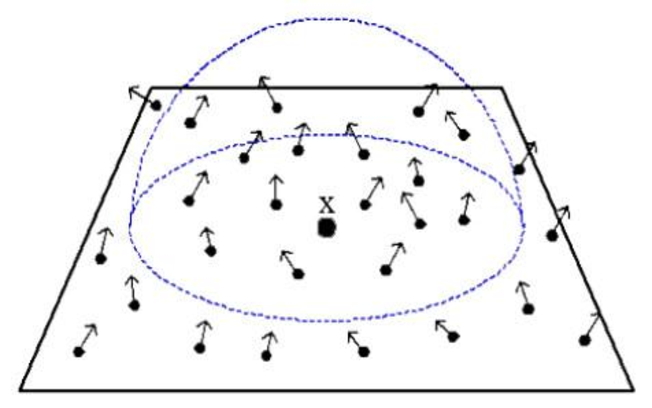
\includegraphics{imgs/photon_density_estimate.pdf}}
    \renewcommand{\thefigure}{\thechapter.\arabic{figure}}
    \caption[Photon Density Estimation Model]{The geometrical setup of photons density estimation.}
    \label{fig:photon_density_estimate}
\end{figure}

\subsection{GPU-based Implementations}
There have already been a couple of successful attempts made to implement global illumination techniques on GPUs. \citeauthor{Purcell:2002:RTP:566654.566640} \cite{Purcell:2002:RTP:566654.566640} presented the first ray tracer entirely running on GPU using a uniform grid for acceleration. \cite{Horn:2007:IKT:1230100.1230129} and \cite{Popov2007} presented the GPU implementations that achieved better performance than a CPU-based ray tracer. With the introduction of general purpose computing on GPU especially with CUDA technology, \citeauthor{Luebke2008} \cite{Luebke2008} presented a technology combining ray tracing and traditional rasterization methods to achieve real-time performance on dynamic scenes.
% TF: Were there any restrictions on how dynamic the scene could be?
Photon mapping has been mapped for multi-core CPUs in \cite{gunther:realtime} and for the older GPU architecture using programmable vertex/pixel shaders in \cite{Purcell:2005:PMP:1198555.1198797}. In the following sections, we will take a look at the techniques that can
be used for performing photon mapping on current GPU hardware with CUDA programming model.

%%%%%%%%%%%%%%%%%%%%%%%%%%%%%%%%%%%%%%%%%%%%%%%%%%%%%%%%%%%%%%%%%%%%%%%%%%

\section{Photon Mapping On GPU using CUDA}

In order to move the photon mapping technique onto graphics hardware, we need to do the creation of traversal of kd-tree on the GPU. The first attempt to achieve this was presented in \cite{Purcell:2005:PMP:1198555.1198797}. However their work was limited by the GPU programming model and hardware architecture.

More general work on parallel kd-tree construction was presented in \cite{popov:06:ESC} and \cite{Shevtsov_highlyparallel}. Both approaches are designed for multi-core CPUs thus are not suitable for GPU. The first problem is that kd-tree construction can easily become bandwidth limited on large input data sets due to its random memory access pattern. Therefore the construction switches from breadth first search (BFS) to depth first search (DFS) manner manner at deeper nodes. This means that these approaches keep the number of concurrently running threads pretty low. GPU hardware, however, is good at having a massive number of threads (at least \(10^{3} - 10^{4}\) running for
%optimal threads\cite{Guide2012}.
% TF: I assume you meant:
optimal performance \cite{Guide2012}.
Another aspect is finding the split position for a node. Both papers use the Surface Area Heuristic (SAH) \cite{springerlink:10.1007/BF01911006} to evaluate the costs for a splitting candidate. Even though the SAH improves kd-tree significantly \cite{wald::PhD}, it is very time consuming.

Finally, parallelizing the photon search or tree traversing is relatively easy, as the tree is accessed read-only. However, for performance reasons it is important that the tree is well balanced and stored efficiently. Storing the tree efficiently means to keep scattered memory accesses as low as possible, by placing child nodes close to their parents. The traversal algorithm itself is not a good candidate for parallelization. Instead, performing multiple traversals simultaneously is a much better way, in order to obtain good performance.

\citeauthor{Zhou2008} presented a new approach to kd-tree construction and traversal on GPUs using CUDA \cite{Zhou2008}. They also provide information on adapting the technique for photon mapping which we will focus on.

\subsection{kd-Tree Construction}
\label{subsec:kdtree_construction}

\citeauthor{Zhou2008} build the kd-tree in BFS manner completely. 
% TF: what is the k in kd-tree? Perhaps give a formal definition of a kd-tree.
During the initialization stage, CUDA's global memory is allocated for the tree construction and the root node is created. For the photon mapping implementation we also have to create three sorted order lists for each dimension for all point coordinates. The points can be grouped into chunks and the bounding box of the node can be computed with segmented reduction.
% TF: Explain "segmented reduction"
Additionally we maintain three associated point ID lists (one for each coordinate axis).

The first stage of construction is called large node stage. In this stage splits nodes using a combination of spatial median splitting and "cutting off empty space" \cite{Havran2000:PhD}. Since in this stage the number of nodes is small, it is better to perform the computation parallelized over all points rather than over nodes. First we need to find the splitting plane (the plane that splits the longest axis in the middle), after repeatedly applying empty space splitting before. Then each photon is classified as being either left (1) or right (0) of the splitting plane. Finally, we perform the scan operation \cite{Mark2007}. After the split we check if the amount of photons in our child nodes is below the threshold \(T = 32\). If the number is smaller, the node is added to the small node list. Otherwise it is added to the active list and scheduled for the next iteration of the large node stage. The large node stage finishes as soon as there are no more nodes in the active list.

The next phase is the small node stage. It begins with a preprocessing step for all nodes in the small node list. In this step we collect all splitting plane candidates and calculate the resulting split sets, which define photon distribution after a split. It should be noted that splitting planes are restricted to initial photon positions in this stage.

After the preprocessing has finished, we process all small nodes in parallel and split them, until each node contains one photon. Since we need to build a kd-tree for points (photons), rather than triangles, we are now using the Voxel Volume Heuristic (VVH) \cite{wald:04:VVH} for split cost evaluation, instead of the SAH \cite{Havran2000:PhD}.

\begin{figure}[ftp]
    \centering
    \fbox{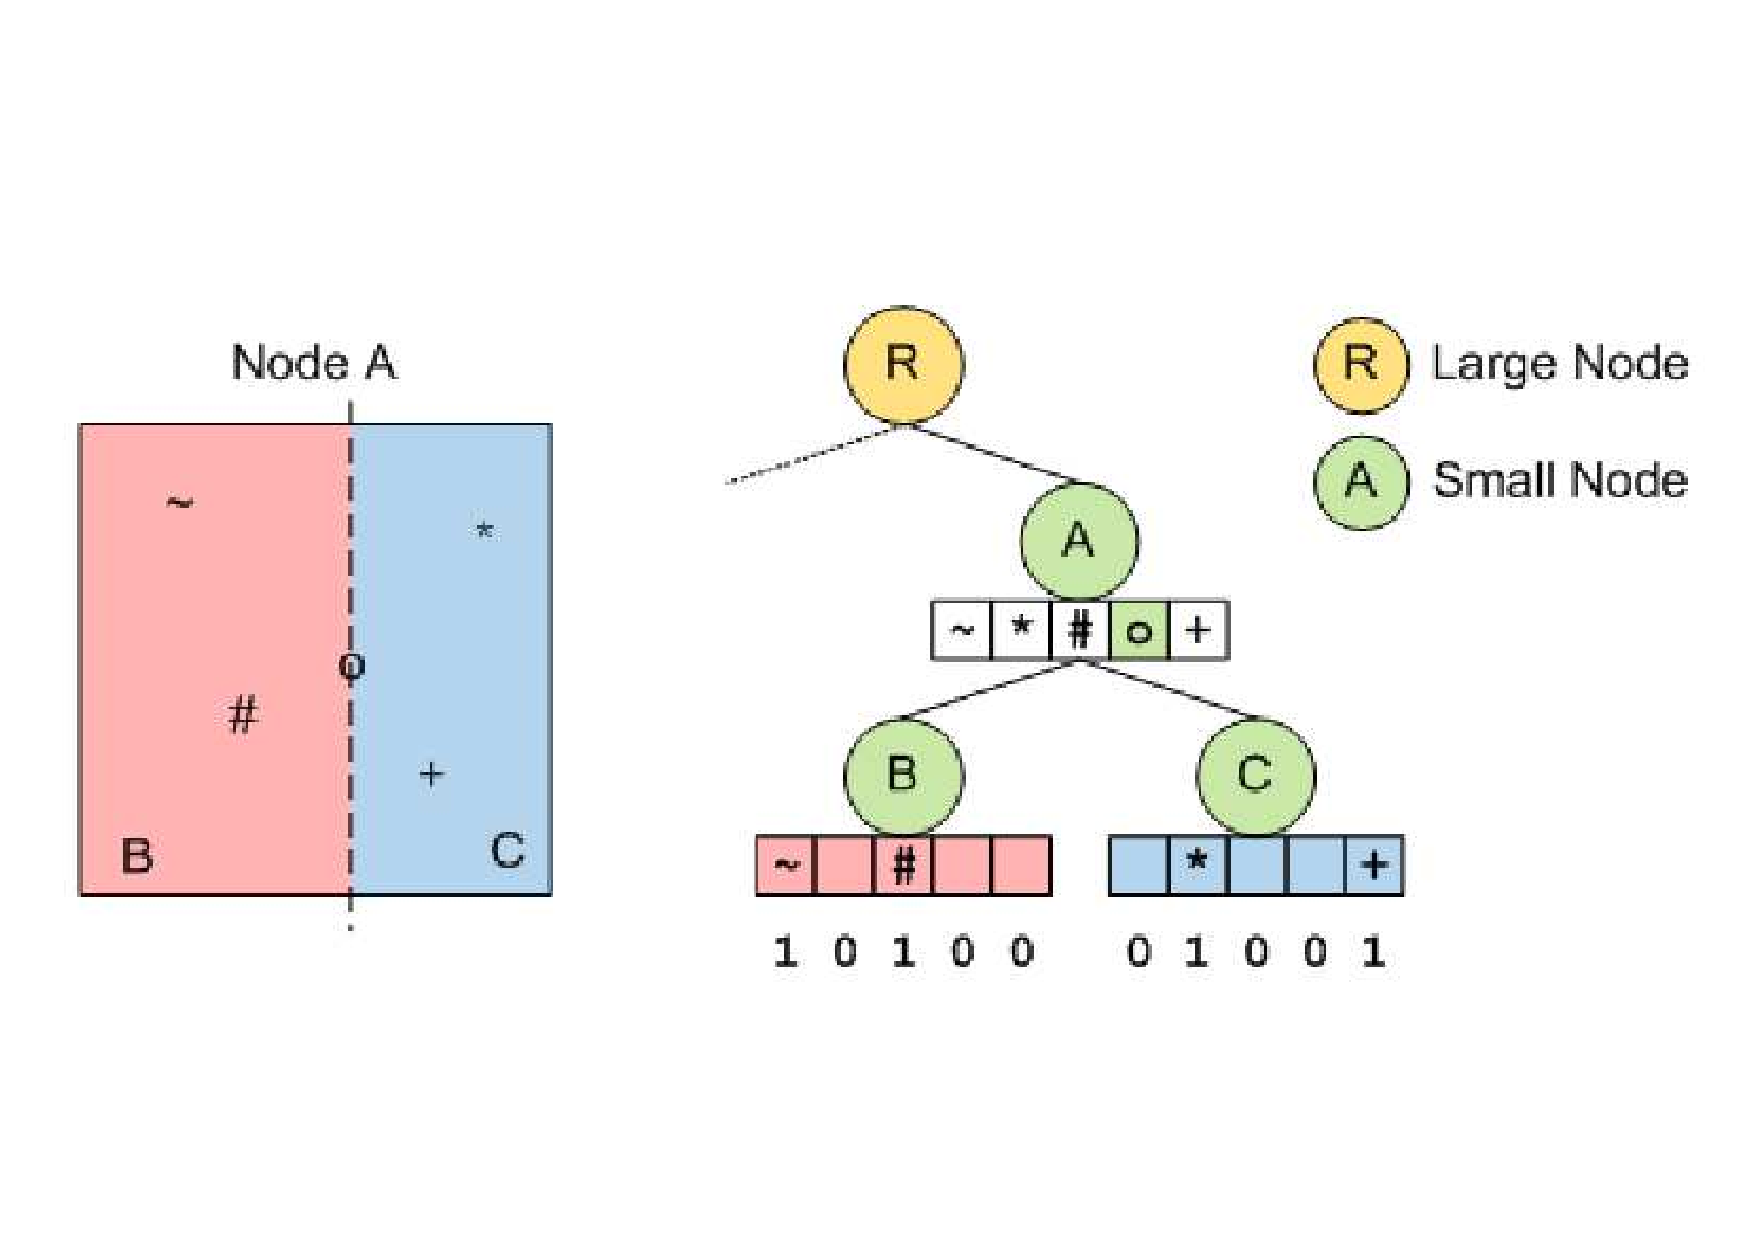
\includegraphics[scale=0.4]{imgs/small_node_stage.pdf}}
    \renewcommand{\thefigure}{\thechapter.\arabic{figure}}
    \caption[The Small Nodes splitting stage within kd-tree construction]{Small node splitting stage following the large nodes  splitting stage in the kd-tree construction process.}
    \label{fig:small_node_splitting}
\end{figure}

After we found the best split candidate (the one with the lowest VVH cost) we can split the small node into two sub nodes. To do so we need the current node's photon set, which is a bit mask representation of the photons inside the node. In order to complete our split, we simply perform a logical AND between the current photon set and the pre-calculated result split sets of the root small node. As illustrated in figure \ref{fig:small_node_splitting}, node A is split into two sub nodes(B and C) and the symbols represent the photons in node A.

Besides easing node splitting, the binary photon representation also helps us calculating the number of photons in a node, which we need for VVH computation and to stop node splitting. All we have to do is to count the bits in the current photon set, using the parallel bit counting routine.

After splitting is done, the new nodes are added to the active node list, in order to be processed during the next iteration step. Of course it can and will happen that some nodes will not create any new child nodes. Therefore, we have to add another step to compact our active node list and remove empty space, as is illustrated in figure \ref{fig:compact_active_list} \cite{Lauterbach09fastbvh}. If there are no more nodes left in the active list, we can finish the small node stage and proceed to the final construction stage.

\begin{figure}[ftp]
    \centering
    \fbox{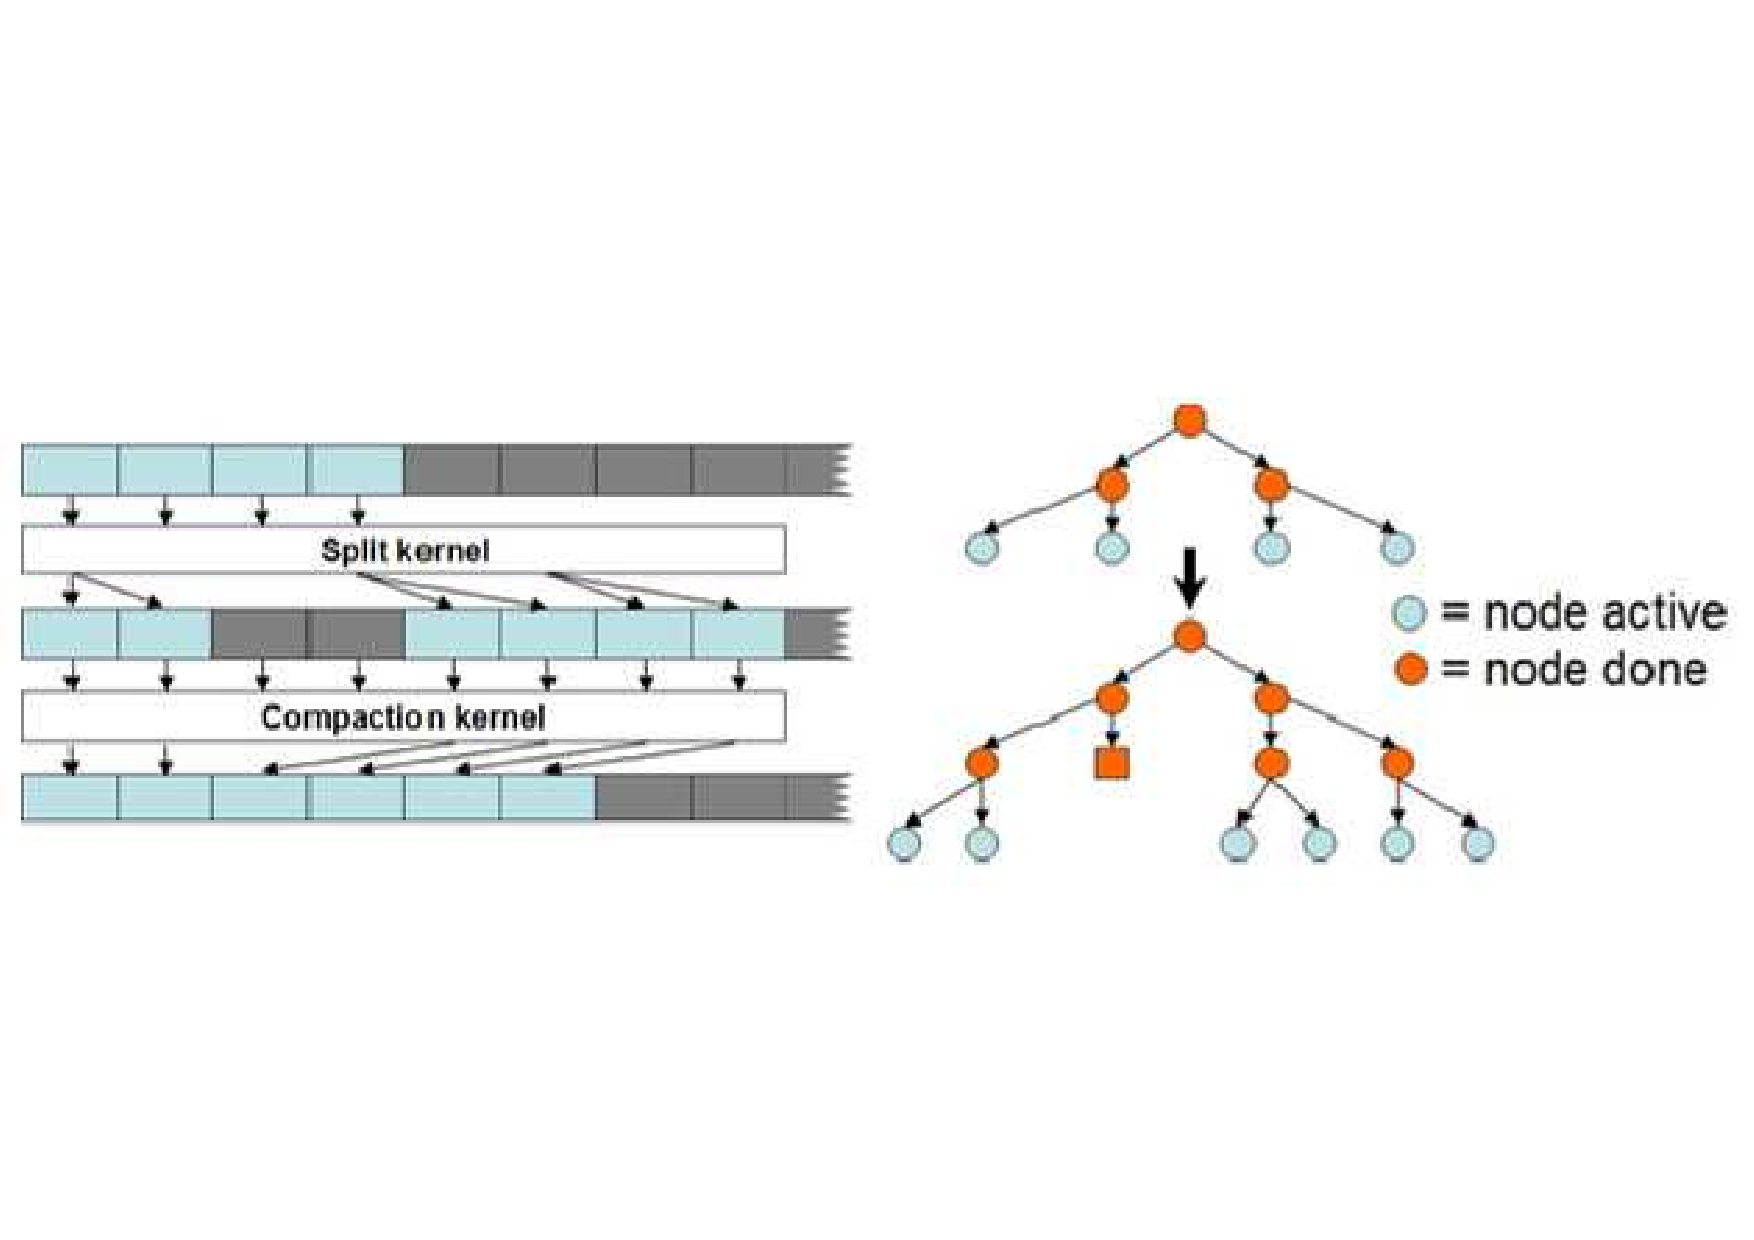
\includegraphics[scale=0.4]{imgs/compact_active_list.pdf}}
    \renewcommand{\thefigure}{\thechapter.\arabic{figure}}
    \caption[Compacting kd-tree nodes in the active node list for next iteration.]{Following the execution of the kernel that splits the kd-tree nodes, a compaction process will be applied on the result nodes in the active node list for the next iteration over the list to build another level of kd-tree.}
    \label{fig:compact_active_list}
\end{figure}

The final stage is the kd-tree output stage, the tree is reorganized to change its layout to a preorder traversal of nodes to improve memory access performance. Firstly we perform a bottom-top traversal to determine the size of the array for preorder tree structure. Then we use another top-down traversal to calculate each node's address and generate tree from sizes. The final output includes the node's bounding box, split plane and the references to its children and the photon's position and power.

\subsection{Photon Search}
In \cite{HenrikWannJensen2004}, Jensen presented a photon searching technique using the priority queue with kd-tree. Unfortunately it is not possible to implement a priority queue with CUDA efficiently since the memory access is incoherent and almost all arithmetic is independent, thus it makes difficult for hardware to hide latency. Therefore \citeauthor{Zhou2008} propose an iterative $K$-Nearest Neighbor (KNN) range search algorithm based on \cite{Preparata:1985:CGI:4333}.
% TF: Perhaps define in some detail what is a KNN range search, especially since it is crucial to your approach..
% TF: Also: how does the K in KNN relate to k in kd-tree? Could be confusing to the reader.

The algorithm starts from an initial conservative search radius \(r_{0}\) and tries to find the query radius \(r_{k}\) through a couple of iterations. For each iteration, a histogram of photon numbers over different radius ranges is created and the final radius is reduced from it. The final radius \(r_{k}\) is then used for range search which returns all photons within that radius. The range search is implemented using the DFS kd-tree traversal algorithm \cite{Preparata:1985:CGI:4333}.

\subsection{Advantages and Limitations}
The GPU approach from \citeauthor{Zhou2008} has a couple of advantages. One is that the KNN search is fast with the worst time complexity of \(O(k\cdot n^{1-\frac{1}{k}})\) \cite{Lee1977}, where \(k = 3\) for a three dimensional kd-tree.
% TF: This k the same as for the kd tree?
Another advantage is the compact data arrangement of the tree giving a space complexity of \(O(n)\).

However this approach also suffers from a couple of limitations. First of all, the dynamic lists are extensively used for storing active nodes, small nodes, final tree nodes and so on and only static arrays are used for optimal performance, therefore additional work has to be done to grow the lists by reallocating the memory and data copying which is expensive operation. To avoid the memory management overhead \citeauthor{Zhou2008} double list sizes when the array need to grow. This leads to increased memory consumption during construction and a big performance hit as we need rebuild the kd-tree for photons every frame. Another limitation is the complexity of implementation, there are too much temporary data to maintain during construction and the requirements of many other data primitive algorithms such as scan, split and sort also increase the complexity of this approach.
